This chapter describes the methods and materials used to address the research questions of the study (Sect.~\ref{s:research_questions}).
Details of the modelling set-up, including initial and boundary conditions are included in this chapter.

\section{Air Quality Modelling} \label{s:modelling}
Models are either Eulerian or Lagrangian, with Eulerian models constituting most of the models used by the AQ modelling community \citep{Russell:2000}.
Eulerian models describe the atmosphere using fixed grid-boxes where species enter in and out of the boxes and the species concentrations are calculated as a function of time. 
While Lagrangian models simulate changes of selected air parcels during advection through the atmosphere, thus there is no exchange between the surroundings and the air parcel (besides emissions) and the model calculates concentrations at different locations and times \citep{Seinfeld:2006}. 

Photochemical models also have different dimensions, ranging from zero-dimensional (box model) to three-dimensional models where the simplicity and computing power increase with model dimension.
Box models are the simplest type of a model having uniform atmospheric concentrations that are only a function of time \citep{Seinfeld:2006}.
Box models lack realism but are extremely useful for studying the detailed processes that influence air quality.
Examples of modelling studies that have used box models include \citet{Bin:2007} and \citet{Noelscher:2014}.

Models numerically solve the chemical species conservation equation describing the processes affecting the concentration of chemical species:
\begin{equation} \label{e:conc}
    \begin{split}
        \frac{\partial c_i}{\partial t} \hspace{2mm} + \hspace{2mm} \nabla \cdot \bar{U}c_i \hspace{2mm} = \hspace{2mm} \nabla \rho D \nabla(c_i/\rho) \hspace{2mm} + \hspace{2mm} R_i(c_1, c_2, \dots, c_n, T, t) \\ + \hspace{2mm} S_i(\bar{x}, t), \hspace{5mm} i = 1, 2, \dots, n.
    \end{split}
\end{equation}
In Eq.~\eqref{e:conc}, $c_i$ is the concentration (in mass or volume) of species $i$, $\bar{U}$ is the wind velocity vector, $D_i$ is the molecular diffusivity of species $i$, $R_i$ is the rate of concentration change of species $i$ through chemical reactions and may be a function of meteorological variables such as temperature.
$S_i(\bar{x}, t)$ is the source or sink of $i$ at location $\bar{x}$, $\rho$ is the air density and $n$ is the number of predicted species.
\citep{Russell:2000}

The dimension and type of model determines the set of differential equations solved at each time step of the model run. 
Numerical methods used to determine the concentration of species $i$ in Eq.~\eqref{e:conc} vary between models, examples include Runge-Kutta \citep{Sandu:1997b}, Finite Element \citep{Russell:2000} or Rosenbrock methods \citep{Sandu:1997a}.

Initial and boundary conditions are required to solve the system of differential equations.
Boundary conditions require knowledge of the concentration and transport of species $i$ at the boundary edges of the model grid.
While initial conditions fix the starting concentration of each species $i$.

\subsection{Model Description and Setup} \label{ss:model_setup}
The MECCA (Module Efficiently Calculating the Chemistry of the Atmosphere) box model was used throughout this work to study the detailed processes influencing the production of ozone.
MECCA was developed by \citet{Sander:2005} and adapted to include MCM~v3.1 chemistry by \citet{Butler:2011}.
The chemical mechanisms used with MECCA in this work are outlined in Sect.~\ref{s:chemical_mechanisms}.
The MECCA box model has been used for studies in modelling of atmospheric gas-phase chemistry including \citet{Kubistin:2010} and \citet{Lourens:2016}.

MECCA is written using the Fortran programming language and runs on UNIX/Linux platforms.
The setup of MECCA that we used uses KPP (Kinetic Pre-Processor) \citep{Damian:2002} to efficiently setup up the system of differential equations for each species considered (Eq.~\eqref{e:conc}).
KPP processes the specified chemistry scheme in the chemical mechanism and generates Fortran code that is then compilied by MECCA.
KPP has many choices of numerical solver for solving the differential equations, a Rosenbrock solver (the ros3 option) throughout this work.

Aside from the chemistry, MECCA also calculates physical parameters at every time step of the simulations.
In our simulations, the pressure, temperature, relative humidity and boundary layer height are held constant at the set values of Table~\ref{t:model_setup}.
\todo[inline]{varying temperature and use of diurnal boundary layer height with vertical mixing in final part of study, latitude and total run time also changed}
\begin{table}[t]%
    \begin{center}%
        \caption{General settings used for MECCA box model in this study.}%
        \begin{tabular}{ll}%
            \hline \hline
            \textbf{Model Parameter} & \textbf{Setting} \\
            \hline \hline
            Pressure & $1013$ hPa \\
            Temperature & $293$ K \\
            Relative Humidity & $81$ \% \\
            Boundary Layer Height & $1000$ m \\
            Latitude & $34\degree$ N \\
            Starting Date and Time & 27th March 06:00 \\
            Model Time Step & $20$ mins \\
            Model Run Time & $7$ days \\
            \hline \hline
        \end{tabular}%
        \label{t:model_setup}%
    \end{center}%
\end{table}%

Photolysis rates in this study are paramaterised as a function of the solar zenith angle.
This paramaterisation requires the degree of latitude for the study to be a defined variable in MECCA, we have chosen the $34\degree$ N latitude which is roughly that of the city of Los Angeles.
and changed to ? in the temperature-ozone study.
The simulations start at the spring equinox (27th March) at 6am and allowed to run for seven diurnal cycles.
or 2 days for final study.

All fluxes of the chemical species into and out of the box are handled by KPP.
The chemical mechanism file includes pseudo-unimolecular reactions specifying the emissions and dry deposition of chemical species with the relevant rate.
The chemical species that are emitted into the model and the emission rates are read into the model using a namelist file.

Namelist files are also used to specify the initial conditions of chemical species and the mixing ratios of those chemical species that are fixed throughout the model.

\section{Chemical Mechanisms} \label{s:chemical_mechanisms}
Chemical mechanisms describe the atmospheric chemistry used by a model.
The chemical mechanism specifies all reactions, products and rate constants of each chemical species.  
The number of species determines the size of the system of differential equations determined by Eq.~\eqref{e:conc} which determines the amount of computing resources required for the model simulations.

Chemical mechanisms range from highly-detailed (explicit) chemical mechanisms to the less-detailed lumped-structure and lumped-molecule chemical mechanisms.
Explicit chemical mechanisms, such as \citet{Aumont:2005}, include thousands of reactions outlining the degradation chemistry of VOCs even including reactions of minor importance in the atmosphere.
Near-explicit chemical mechanisms, such as the Master Chemical Mechanism (MCM) of \citet{Jenkin:1997}, \citet{Jenkin:2003}, \citet{Saunders:2003}, \citet{Bloss:2005} are less-detailed than explicit chemical mechanisms but still contain thousands of reactions and as such are mainly used in box models.
%The MCM representation of VOC degradation chemistry is discussed in more detail in Sect.~\ref{ss:near_explicit}.

Many other chemical mechanisms developed simplified approaches to describe atmospheric chemistry for use in regional and global models.
These reduced chemical mechanisms aggregate (or lump) VOC into mechanism species and the secondary degradation of these mechanism species attempts to replicate ambient measurements and chamber experiments \citep{Stockwell:2012}.
The first part of this study compares the maximal ozone produced from a number of reduced chemical mechanisms, listed in Table~\ref{t:mechanisms}, a description of the different reduction techniques used by the reduced mechanisms is found in Sect.~\ref{ss:lumped_intermediate}, Sect.~\ref{ss:lumped_molecule} and Sect.~\ref{ss:lumped_structure}.
The main results from the chemical mechanism comparison study are presented in Sect.~\ref{s:chemical_mechanism_results}.
\todo[inline]{see about wording and less repetition to intro}
\begin{table}[t]%
    \begin{center}%
        \caption{Chemical mechanisms used in the study.}%
        \scalebox{.85}[.85]{\begin{tabular}{lll}%
                \hline \hline
                \textbf{Chemical Mechanism} & \textbf{Lumping Type} & \textbf{Reference} \\
                \hline \hline
                \multirow{3}{*}{MCM v3.1 and v3.2} & \multirow{3}{*}{No lumping} & \citet{Jenkin:1997}, \citet{Jenkin:2003} \\
                & & \citet{Saunders:2003}, \citet{Bloss:2005} \\
                & & \citet{MCM_Site} \\
                CRIv2 & Lumped intermediates & \citet{Jenkin:2008} \\
                MOZART-4 & Lumped molecule & \citet{Emmons:2010} \\
                RADM2 & Lumped molecule & \citet{Stockwell:1990} \\
                RACM & Lumped molecule & \citet{Stockwell:1997} \\
                RACM2 & Lumped molecule & \citet{Goliff:2013} \\
                CBM-IV & Lumped structure & \citet{Gery:1989} \\
                CB05 & Lumped structure & \citet{Yarwood:2005} \\
                \hline \hline
            \end{tabular}%
        }%
        \label{t:mechanisms}%
    \end{center}%
\end{table}%

\subsection{Near-Explicit Chemical Mechanisms} \label{ss:near_explicit}
The Master Chemical Mechanism (MCM~v3) is a near-explicit mechanism describing the chemical degradation of 107 non-aromatic VOCs in \citep{Saunders:2003} and 18 aromatic VOCs in \citep{Jenkin:2003}. 
The MCM~v3.2 was the reference mechanism throughout this study as it was the most recent version of the MCM at the time of the first experiments related to the chemical mechanism study; the MCM~v3.2 was obtained from the world wide web (\mbox{\url{http://mcm.leeds.ac.uk/MCMv3.2/}}).
In total, the MCM~v3.2 has $12,691$ reactions including $4351$ organic compounds and $46$ inorganic compounds. 
%The primary VOCs represented by the MCM~v3.2 were determined by which VOC have the most emissions (by mass) as listed by the UK National Atmospheric Emissions Inventory and makes up about 70\% of the mass emissions of unique species achieved.

Rate constants and branching ratios of the reactions represented in the MCM~v3.2 are those recommended by IUPAC.
If no data was available then they are estimated using structure activity representation (SAR) or group reactivity (GR) methods.
Each primary VOC and each degradation product, is individually degraded until it is broken down to \ce{CO2}, \ce{H2O}, CO or an organic product (or radical) already represented by the MCM \citep{Jenkin:1997}. 
In order to minimize the number of reactions and species in the MCM~v3, reactions with low probability and those reactions deemed of minor importance are not included.
Also the reactions between peroxy radicals are represented by a single parameterised reaction which greatly reduces the number of reactions.
\begin{figure}%
    \begin{center}%
        \caption[Flowchart of VOC degradation represented by the MCM]{Flowchart of the major reactions of primary VOCs, intermediates and products considered in the MCM. Figure~1 in \citet{Saunders:2003}}%
        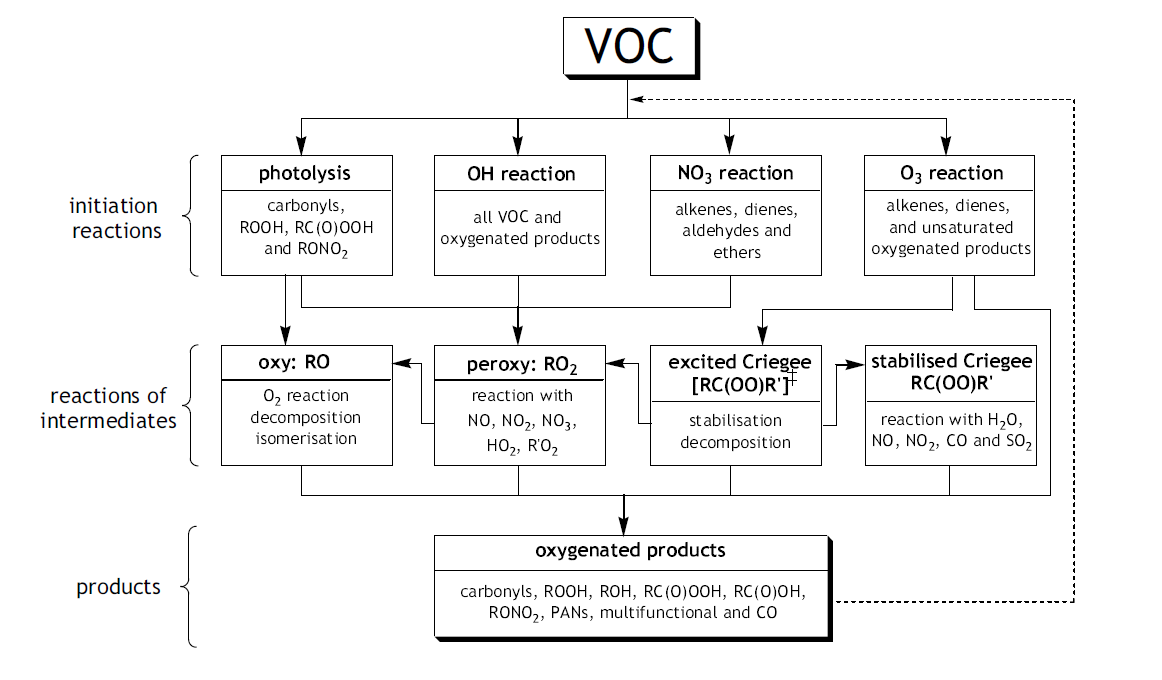
\includegraphics[width=\textwidth]{MCM_scheme.png}
        \label{f:MCM_scheme}%
    \end{center}%
\end{figure} %

\subsection{Lumped Intermediate Chemical Mechanisms} \label{ss:lumped_intermediate}
Lumped intermediate chemical mechanisms aggregate the degradation products rather than primary VOC.
The Common Representative Intermediates (CRI) chemical mechanism \citep{Jenkin:2008} is an example of a lumped intermediate mechanism.

The CRI is a reduced version of the MCM developed for 3-D models.
Reducing the complexity of the MCM was achieved by representing many degradation products (intermediates) in the CRI by a single mechanism species designed to produce the same amount of ozone as when using the MCM.
The CRI~v2 was used in this study and the intermediates in this version of the CRI mirror the ozone production from the MCM~v3.1.

The CRI~v2 is available online (\mbox{\url{http://mcm.leeds.ac.uk/CRI}}) in a full version and further reduced variants that include even further reductions to the chemistry represented in MCM~v3.1 by also lumping VOCs into lumped mechanism species.
\citet{Jenkin:2008} describes the main assumptions made in order to condense the organic chemistry of the MCM~v3.1 to the lumped intermediate chemistry of the CRI~v2, while \citet{Watson:2008} describes the further reductions made to the CRI~v2 to produce the five lumped emission variants.
The most reduced version of the CRI~v2 has also been implemented into the widely used 3-D regional model WRF-CHEM \citep{Archer-Nicholls:2014}.

\subsection{Lumped Molecule Chemical Mechanisms} \label{ss:lumped_molecule}
Lumped molecule chemical mechanisms aggregate primary VOC into mechanism species and is the most simplification common technique.
However, lumped-molecule chemical mechanisms use different approaches in creating these lumped species.
Typically VOCs having large emissions, such as methane, isoprene, ethane and ethene, are represented by dedicated species with mechanism species used to represent all other VOCs.
These lumped mechanism species typically represent NMVOC based on functional group, OH-reactivity or a combination of both.
Table~\ref{t:mechanisms} lists the lumped-molecule chemical mechanisms used in this thesis and implemented into the MECCA model.

\subsubsection{MOZART}
The Model for OZone and Related chemical Tracers (MOZART) chemical mechanism is an example of a lumped molecule chemical mechanism used in global and regional 3-D models.
MOZART was developed for global chemical transport models and describes chemical processes within the planetary boundary layer, free troposphere and stratosphere.
MOZART-4 \citep{Emmons:2010} was used in this study.

MOZART-4 represents methane, ethane, propane, ethene, propene, isoprene and formaldehyde by explicit species.
The lumped mechanism species, BIGALK, BIGENE and TOLUENE, are used to represent alkanes and alkenes with four or more carbon atoms and all aromatic VOC \citep{Emmons:2010}.
Thus, the lumping species used by MOZART are based on the functionality of the VOC.
There are no mechanism species representing emissions of esters, ethers or chlorinated NMVOC, when representing emissions of these less-reactive NMVOC are added to the BIGALK mechanism species as this has the lowest OH-reactivity.

\todo[inline]{modifications for use in MECCA}

\subsubsection{RADM2}
The Regional Acid Deposition Model (RADM2) \citep{Stockwell:1990} is used in regional modelling studies.
RADM2 is still popular within the modelling community as outlined by the review of European modelling groups by \citet{Baklanov:2014}.

Methane, ethane, ethene, isoprene and formaldehyde are represented explicitly in RAMD2.
RADM2 represents other VOC using lumped species based on the OH-reactivity and functional group of the VOC.
The lumped mechanism species, HC3, HC5, and HC8, represent alkanes and other VOCs such as alcohols, ethers and  chlorinated VOC based on their OH-reactivity.
Alkenes are represented by OLT or OLI depending on the position of the double bond (OLT: terminal alkenes and OLI: internal alkenes).

Aromatic VOC are represented by TOL or XYL depending on OH-reactivity and CSL is used for hydroxy-substituted aromatics.
Carbonyls and organic acids are also represented by lumped mechanism species.
Typically the NMVOC having the least number of carbons (e.g. formaldehyde and formic acid) is represented by an explicit species and then all other species from that functional group are represented by a lumped species.

\subsubsection{RACM}
\citet{Stockwell:1997} describes Regional Atmospheric Chemistry Mechanism (RACM) which updates RADM2.
RACM includes further lumped mechanism species such as API and LIM to represent cyclic terpenes with one double bond and all other cyclic terpenes.

\subsubsection{RACM2}
RACM was further extended and updated to RACM2 \citep{Goliff:2013} including more lumped mechanism species to represent primary VOC emissions as well as updating the secondary chemistry of lumped mechanism species.
The biggest changes in the chemistry was to the representation of aromatic chemistry.
RACM2 now represents aromatic VOC using eight mechanism species instead of three species as in RACM, with explicit representation of benzene and each xylene isomer having its own mechanism species.
The secondary chemistry of the aromatic VOC was updated to reflect the MCM.

Acetone and methyl ethyl ketone (MEK) are now treated as separate species rather than being represent as a single mechanism species, KET, in RADM2 and RACM.
Alcohols are also represented in RACM2, whereas in the previous versions, alcohols were represented by HC3, HC5 or HC8.
\todo[inline]{isoprene degradation products from RADM2->RACM->RACM2}

\subsection{Lumped Structure Chemical Mechanisms} \label{ss:lumped_structure}
Lumped-structure chemical mechanisms express VOCs as permutations of building blocks representing the structure of the emitted VOC.
The Carbon Bond mechanism is the most widely used lumped-structure chemical mechanism which includes mechanism species representing the different carbon bonds present in emitted VOC.

\subsubsection{CBM-IV}
The fourth version of the Carbon Bond mechanism was developed to represent the chemistry in polluted urban conditions and described in \citet{Gery:1989}.
CBM-IV represents $20$ organic species and requires $46$ reactions to fully represent the secondary chemistry.
Explicitly represented emitted NMVOC are those with the most significant emissions: isoprene, ethene and formaldehyde.
Mechanism species represent the \ce{C-C} bond (PAR), OLE represents \ce{C=C} and ALD2 represents \ce{C=O} and less and more reactive aromatic VOC are represented by TOL and XYL. 

NMVOC emissions emitted by the mechanism species are described in \citet{Hogo:1989}.
For example, if heptane, having seven carbons each with a single bond, has emissions of $1 \times 10^9$~molecules~cm$^{-3}$~s$^{-1}$ then using the CBM-IV, these emissions would be represented by $7$~PAR and thus PAR emissions would be $7 \times 10^9$~molecules~cm$^{-3}$~s$^{-1}$.
Also, propene is represented as $1$~OLE and $1$~PAR and so emissions of $1 \times 10^9$~molecules~cm$^{-3}$~s$^{-1}$  would be emitted as $1 \times 10^9$~molecules~cm$^{-3}$~s$^{-1}$ of OLE and $1 \times 10^9$~molecules~cm$^{-3}$~s$^{-1}$ of PAR.

\subsubsection{CB05}
CBM-IV was updated to CB05 \citep{Yarwood:2005} to include more species representing emitted VOC.
CB05 includes $99$ organic reactions to represent the degradation of $37$ organic species.
Mechanism species for terpenes (TERP), ethane (ETHA), aldehydes with more than three carbons (ALDX), methanol (MEOH), ethanol (ETOH) and alkenes with both internal (IOLE) and external (OLE) double bonds were included.  
CB05 was also updated to include low-\ce{NO_x} chemistry including peroxide formation.

\section{Using the Chemical Mechanisms in MECCA}
Each chemical mechanism listed in Table~\ref{t:mechanisms} was adapted to the KPP format for use in the MECCA box model.
The WRF-Chem model \citep{Grell:2005} includes KPP versions of RADM2, RACM and CBM-IV and was the starting point for using these chemical mechanisms in MECCA.
The chemistry specified by the original reference was adapted to the KPP format for all other chemical mechanisms.

The inorganic chemistry of the MCM~v3.2 was used in each chemical mechanism to focus on differences between the representation of secondary degradation chemistry in the chemical mechanisms.
The photolysis parameterisation used by the MCM~v3.2 was also used in each chemical mechanism.
Finally, the MCM~v3.2 approach to peroxy-peroxy reactions was also used in each chemical mechanism.
Further details of these changes are found in the supplementary material of the first paper of this thesis (Chap.~\ref{c:paper_1}). 
\todo[inline]{Include supplementary material}

\section{Initial and Boundary Conditions}
In all simulations, methane (\ce{CH4}) was fixed to $1.75$~ppmv while carbon monoxide (CO) and \ce{O3} are initialised at $200$~ppbv and $40$~ppbv and then allowed to evolve freely.
The initial conditions for all NMVOCs was held constant until noon of the first day of simulations to simulate a fresh plume of emissions.

The initial conditions for NMVOC species differed in each experiment.
In the first study, comparing the effects of different VOC secondary degradation on ozone production, the initial conditions used in \citet{Butler:2011} were used.
The study of \citet{Butler:2011} introduced the Tagged Ozone Production Potential (TOPP), described further in Sect.~\ref{s:tagging}, by considering the degradation of VOCs typical of Los Angeles and Beijing using MECCA setup with MCM~v3.1 chemistry.
The same initial conditions of the Los Angeles experiments in \citet{Butler:2011} were used in the MECCA set-up with MCM~v3.2 chemistry.
This model setup was used to determine the emissions needed for constant mixing ratios of the NMVOCs.
These emissions were mapped to the appropriate chemical species of each chemical mechanism in Table~\ref{t:mechanisms} keeping amount of emitted NMVOC constant between model setups.
Results of this comparison are presented in Sect.~\ref{s:chemical_mechanism_results}.

The second study looked at the sensitivity of different speciations of NMVOC emissions from emission inventories of the solvent sector on ozone production.
Table~\ref{t:solvent_speciations} lists the solvent sector speciations used in this study.
This study considered a theoretical urban area of $1000$~km$^2$ with total NMVOC emissions of $1000$~tons/day.
The solvent sector contributes $\sim43$~\% by mass of total emissions \citep{AQEU:2011}, thus total NMVOC emissions of $430$~tons/day were used.
\begin{table}[t]%
    \begin{center}%
        \caption{The solvent sector emission inventories compared in this study.}%
        \begin{tabular}{lllP{5.2cm}}%
            \hline \hline
            \textbf{Speciation} & \textbf{Comment} & \textbf{Reference} \\ 
            \hline \hline
            TNO & European average &  \citet{Builtjes:2002} \\ \hline
            IPCC & Model Specific & \citet{Ehhalt:2001} \\ \hline
            EMEP & Model Specific & \citet{Simpson:2012} \\ \hline
            DE94 & Country Specific & \citet{Friedrich:2002} \\ \hline
            GR95 & Country Specific & \citet{Sidiropoulos:2007} \\ \hline
            GR05 & Country Specific & \citet{Sidiropoulos:2007} \\ \hline
            UK98 & Country Specific & \citet{Goodwin:2000} \\ \hline
            UK08 & Country Specific & \citet{Murrells:2010} \\ 
            \hline \hline
        \end{tabular}%
        \label{t:solvent_speciations}%
    \end{center}%
\end{table}%

The total NMVOC emissions of the solvent sector were mapped to MCM~v3.2 species based on the speciations of each emission inventory in Table.~\ref{t:solvent_speciations}.
Model simulations were repeated using MOZART-4 and RADM2 to investigate whether changing the chemical mechanism affects the differences in ozone concentrations between the solvent sector emission inventories.
Further simulations using total emissions of $1000$~tons/day while varying the speciation of just the solvent sector emissions were also performed.
In these simulations, the TNO speciation for all other (non-solvent use) source sectors was used.
Further simulations adding emissions of biogenic VOCs, in this case we considered only isoprene and monoterpenes, were included using the European average contribtion of BVOC emissions specified by EMEP \citep{Simpson:2012}.
Details are also detailed in Sect.~\ref{s:EI_results}.

The final study looked at the ozone-temperature relationship over central Europe and the emissions of NMVOC over Benelux (Belgium, Netherlands and Luxembourg) were used.
The TNO\_MACCIII emissions for the year 2011 were used as anthropogenic NMVOC emissions and mapped to MCM~v3.2 species.
Temperature indepedent emissions of the biogenic species isoprene and monoterpenes were again taken from EMEP speciation for Benelux \citep{Simpson:2012}.
In simulations using temperature-dependent emissions of isoprene, the Model for Emissions of Gases and Aerosols from Nature (MEGAN2.1) \citep{Guenther:2012} algorithm was used.
All simulations were repeated using CRI~v2, MOZART-4, RADM2 and CB05 chemistry.
Sect.~\ref{s:T-O3_results} includes further details.

The first two studies, comparing different chemical mechanisms and solven speciations, used \ce{NO_x} conditions generating VOC-and-\ce{NO_x} sensitive chemistry.
This was achieved by emitting the amount of NO required to balance the source of radicals at each time step.
This calculation was performed online during the model simulations by including new code in the model.

The final study assessed the relationship between ozone and temperature using different \ce{NO_x} conditions.
For these simulations, a constant source of NO emissions was systematically varied between $5.0~\times~10^9$ and $1.5~\times~10^{12}$~molecules~(NO)~cm$^{-2}$~s$^{-1}$.

The setup of the boxmodel in the first two studies was a contained box with no exchange out of the box, thus no chemical boundary conditions were required.
MECCA was updated for the final study to include a diurnal profile of the PBL and included mixing into the free troposphere.
The diurnal profile included in the model was that measured during the BAERLIN2014 campaign \citep{Bonn:2016}.
Free troposphere mixing ratios for \ce{O3}, \ce{CH4} and CO were set to $50$~ppbv, $1.8$~ppmv and $116$~ppbv respectively. 
These mixing ratios were taken from the $700$~hPa height using the MATCH-MPIC chemical weather forecast data from March~21st.

\section{Tagging the Chemical Mechanisms} \label{s:tagging}
One of the strengths of atmospheric modelling is the ability to allocate ozone production to sources.
Many techniques have been used to perform this, for example comparing ozone levels with and without emissions from a type of VOC or froma particular sector such as in \citet{Butler:2012}. 
\todo[inline]{example Tim megacity? improve bibtex}
Tagging is another approach, in this approach the chemical mechanism is modified to include chemical species including a label (the tag) indicating the source category or other information.
For example, MOZART-4 includes tagged chemistry that allows attribution of ozone production to categories of \ce{NO_x} emissions \citep{Emmons:2012}. \todo{update bibtex}

\citet{Butler:2011} introduced tagging of NMVOC chemistry that allows ozone production to be allocated to emitted NMVOC.
This approach was used in conjunction with VOC-\ce{NO_x}-chemistry to determine the maximum ozone production potential of different NMVOC, called the Tagged Ozone Production Potential (TOPP).
The TOPP allocated production of \ce{O_x}, the chemical family including \ce{O3}, \ce{NO2} and other chemical species involved in fast cycles of production and loss with \ce{O3} or \ce{NO_x}, to emitted NMVOC by counting the number of NO to \ce{NO2} converions by each peroxy radical produced during the degradation of an NMVOC through \eqref{r:RO2_NOb}.

The calculation uses \ce{O_x} production as a proxy for \ce{O3} production and \citet{Butler:2011} showed that this allocation is only valid for \ce{NO_x}-limited and VOC-and-\ce{NO_x} sensitive chemistry not in conditions with high \ce{NO_x} conditions.
The tagging described in \citet{Butler:2011} for MCM~v3.1 chemistry was processed for use with all the chemical mechanisms in Table~\ref{t:mechanisms}.
As the first two studies use VOC-and-\ce{NOx}-sensitive conditions, model simulations using the tagged versions of the chemical mechanisms were performed to aid in analysing the results.
In the first study, the tagging approach was used to compare the secondary degradation of emitted NMVOC and in the second study, tagging was used to analyse and attribute \ce{O_x} production to the emitted NMVOCs specified by the solvent speciations in Table~\ref{t:solvent_speciations}.

The variable \ce{NO_x} conditions used in the third study meant that using the tagging approach was not possible.
Thus all model simulations assessing the ozone-temperature relationship with different \ce{NO_x} conditions were performed with non-tagged versions of the chemistry.
The possibility of tagging VOC chemistry that is appropriate for use in all NOx conditions would be an asset for many modelling studies.
\todo[inline]{possible citation for this??}
